\chapter{构建验证与结论展望}\label{chap:build-validation}

系统移植是否完成，需要通过可重复的构建流程和可观察的运行结果确认。当前系统需要编译 Rust 内核，交叉编译 C 用户库、Shell 和用户程序，生成包含内核、用户程序和文件系统内容的磁盘镜像，并通过 QEMU RISC-V virt 机器启动到可交互 Shell。本章说明文件设备交互环境、构建与运行方式、功能测试范围和结果分析，并在最后总结本文工作与后续完善方向。

\section{文件、设备与 Shell 交互环境}

文件系统、块设备、字符设备和 Shell 共同构成了用户能够直接观察到的系统环境。用户向终端输入命令后，字符设备和 TTY 层负责接收输入，Shell 解析命令并通过系统调用访问文件、创建进程或建立管道；文件读写最终通过文件系统、缓冲区和块设备到达磁盘镜像。本节只说明文件系统和 Buffer 管理在当前系统集成路径中的接口作用，不展开 inode 分配、目录项维护、缓冲区替换等细节；重点放在 RISC-V/QEMU 平台下设备模型的变化，以及 TTY 和 Shell 如何与前文的系统调用、进程管理机制连接。

当前系统保留 Unix V6++ 的文件系统接口和主要用户态语义，包括超级块、inode、目录项、打开文件表、当前工作目录以及 \verb|open|、\verb|read|、\verb|write|、\verb|creat|、\verb|link|、\verb|unlink|、\verb|chdir|、\verb|stat|、\verb|dup| 和 \verb|pipe| 等系统调用。内核启动阶段调用 \verb|load_file_system| 读取根设备超级块，调用 \verb|init_root_directory| 取得根目录 inode，并为 0 号进程的 \verb|Userspace| 设置当前目录。随后，系统通过 \verb|kernel_open| 打开 \verb|/dev/tty1|，把文件描述符 0 和 1 绑定到控制台输入输出，为 Shell 交互建立基本环境。

相较原 \verb|main| 分支，文件系统的外部行为尽量保持稳定，资源引用方式则更偏向 Rust 的所有权模型。当前代码使用 \verb|InodeRef|、\verb|FileRef|、\verb|InodeRefGuard| 等类型封装 inode 和文件对象的引用关系，克隆引用时增加表项计数，离开作用域时通过 \verb|Drop| 归还引用。原 C++ 版本通常在调用路径中显式执行 \verb|IGet|、\verb|IPut|、\verb|CloseF| 等操作；当前版本保留这些 Unix 风格的表结构概念，并把一部分成对操作收束到引用类型的生命周期中。教学上仍可观察文件表和 inode 表，调用者忘记释放引用的机会也相应减少。

原 IA-32/C++ 版本运行于 PC 机器模型，块设备主要面向 ATA/IDE 硬盘，驱动代码需要直接操作 I/O 端口、LBA28 寄存器、DMA 描述符和 8259A 中断结束命令。当前 RISC-V/Rust 版本面向 QEMU virt 机器，块设备改为 VirtIO MMIO 设备。内核通过 \verb|VirtIOBlockDriver::find_block_device| 扫描 virt 机器提供的 MMIO slot，识别 VirtIO Block 设备后建立驱动对象；读写请求通过 \verb|virtio-drivers| 库提交给设备，并以 512 字节扇区为单位访问磁盘镜像\cite{qemu_riscv_doc,virtio_1_2}。上层文件系统继续通过 \verb|bread|、\verb|bwrite|、\verb|bdwrite| 等缓冲区接口访问块数据，磁盘后端迁移后，上层接口基本保持稳定。

\begin{figure}[htbp]
  \centering
  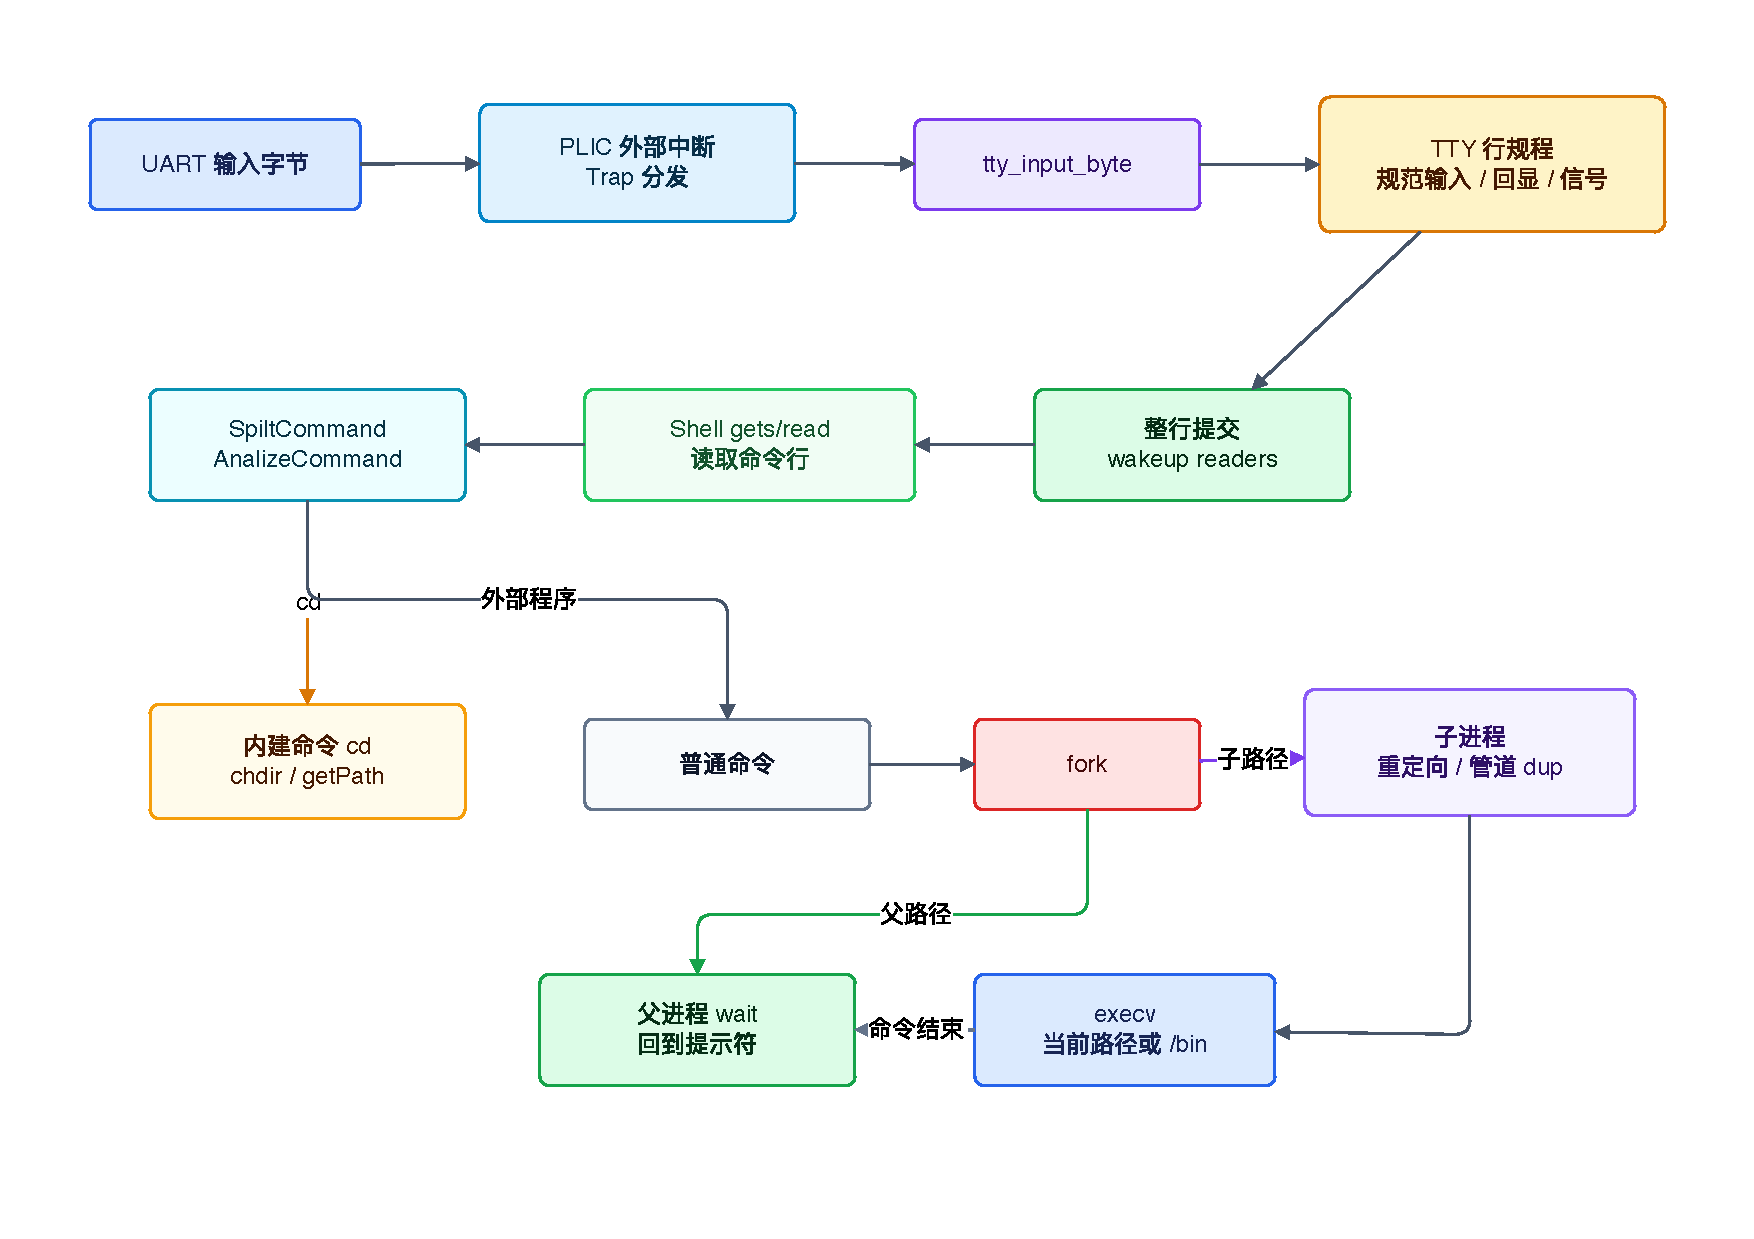
\includegraphics[width=0.95\textwidth]{figures/tty-shell-flow.pdf}
  \caption{终端输入到 Shell 执行的交互路径}\label{fig:tty-shell-flow}
\end{figure}

\figref{fig:tty-shell-flow} 展示了从输入字节到命令执行的路径。TTY 默认工作在规范输入模式，用户输入一行并按下回车后，因 \verb|read| 等待的 Shell 被唤醒。Shell 的 \verb|main1| 输出提示符，调用 \verb|gets| 读取命令行，再通过 \verb|SpiltCommand| 和 \verb|AnalizeCommand| 构造命令树。内建命令 \verb|cd| 由 Shell 直接调用 \verb|chdir| 并更新当前路径；普通命令则先 \verb|fork|，子进程完成输入输出重定向或管道描述符复制后，尝试执行当前路径下的程序，失败后再尝试 \verb|/bin| 目录下的同名程序。

TTY 层还与信号机制相连接。当输入字符等于中断、退出或挂起控制字符时，TTY 会根据 \verb|Termios| 配置回显控制字符，并通过进程管理器向相关进程发送 \verb|SIGINT|、\verb|SIGQUIT| 或 \verb|SIGTSTP|。用户可以由此在终端中观察信号递送效果。原 C++ 版本的 TTY 直接面向键盘和显示输出路径，当前版本把输入输出收束到 UART 串口和 Console 字符设备，更符合 QEMU virt 的无图形运行方式。

\section{构建与运行环境}

当前仓库采用 Makefile 组织整体构建，用 Cargo 构建 Rust 内核，用 RISC-V 交叉 GCC 构建用户态 C 程序。内核部分在 \verb|src/Makefile| 中调用 \verb|cargo +nightly-2026-04-07 rustc|，目标三元组为 \verb|riscv64gc-unknown-none-elf|，并使用 \verb|-Z build-std=core,alloc,compiler_builtins| 构建裸机所需的标准库子集。Cargo 输出静态库后，Makefile 再用 \verb|rust-lld| 和 \verb|src/kernel-riscv64.ld| 链接生成 \verb|src/kernel.elf|。这种流程与普通用户态 Rust 程序不同，原因在于内核运行在无标准库、无操作系统服务的环境中，只能使用 \verb|core|、\verb|alloc| 和明确接入的底层库。

用户态部分仍由 C 语言实现。用户库 \verb|lib/libv6pptongji.a|、Shell 的 \verb|Shell.exe| 以及 \verb|programs| 目录下的 \verb|ls|、\verb|cat|、\verb|echo|、\verb|cp|、\verb|rm|、\verb|mkdir|、\verb|fork|、\verb|sig| 等程序都通过 \verb|riscv64-unknown-elf-gcc| 编译，并使用 \verb|-march=rv64gc|、\verb|-mabi=lp64d|、\verb|-ffreestanding|、\verb|-nostdlib| 等选项生成独立的 RISC-V ELF64 可执行文件。链接时指定 \verb|-Ttext-segment=0x400000| 和入口 \verb|_start|，与第 3 章中的 ELF 加载地址和用户态 C 运行时入口相对应。

\begin{figure}[htbp]
  \centering
  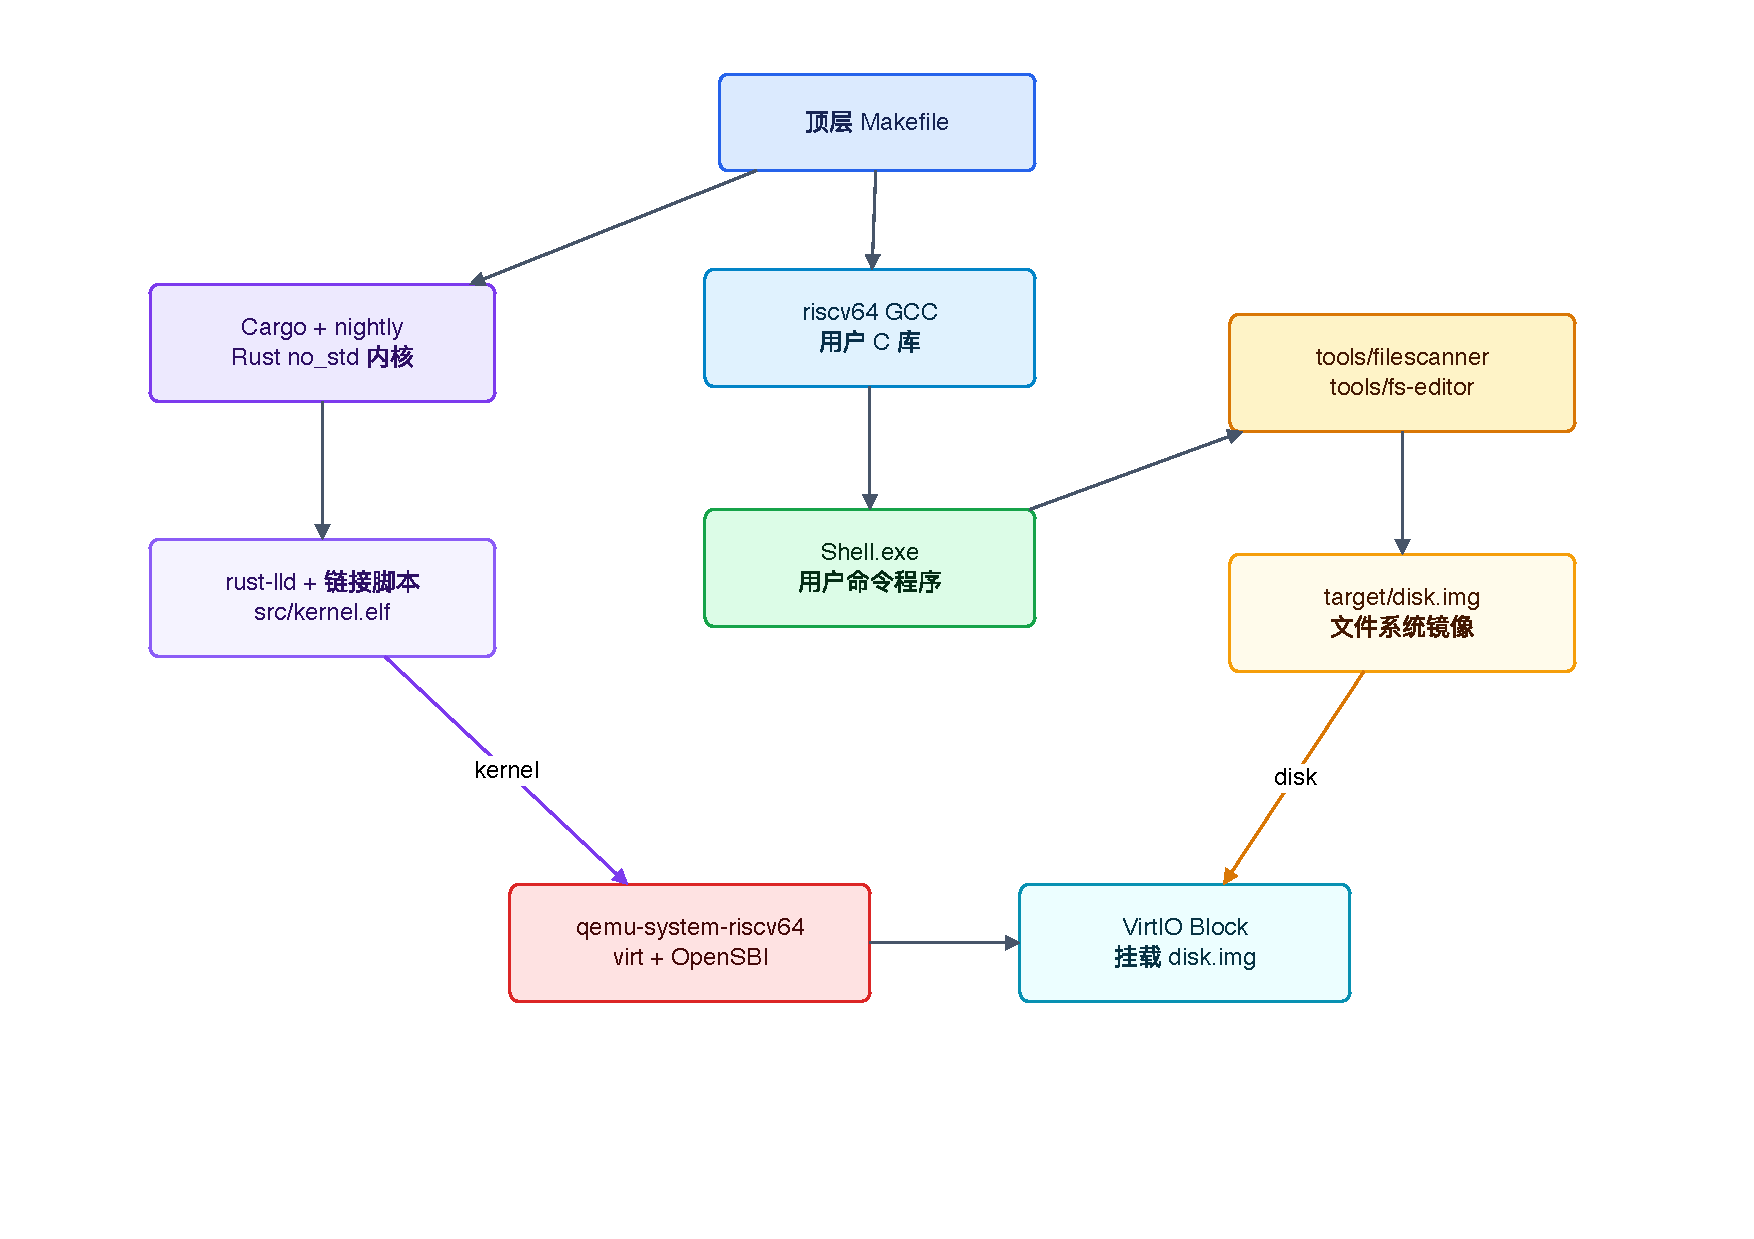
\includegraphics[width=0.95\textwidth]{figures/build-pipeline.pdf}
  \caption{内核、用户程序与磁盘镜像构建流程}\label{fig:build-pipeline}
\end{figure}

\figref{fig:build-pipeline} 展示了当前构建流程。顶层 \verb|make all| 依次构建工具、用户库、Shell、用户程序和内核，并将构建产物复制到 \verb|target/img-workspace|。随后，\verb|tools/filescanner| 扫描工作目录内容，\verb|tools/fs-editor| 生成 \verb|target/disk.img|。运行 RISC-V 目标时，\verb|make qemu-riscv64| 使用 \verb|qemu-system-riscv64|、\verb|-machine virt|、\verb|-bios default|、\verb|-nographic| 和 \verb|-kernel src/kernel.elf| 启动内核，同时通过 VirtIO MMIO 设备挂载 \verb|target/disk.img| 作为块设备后端\cite{qemu_riscv_doc}。

相较 \verb|main| 分支，构建和运行对象发生了三类变化。原版本主要通过 CMake/Ninja 构建 C++ 内核，并通过 \verb|qemu-system-i386| 和 IDE 磁盘启动；当前版本增加 Rust 内核构建链和 RISC-V 运行目标。原用户态程序主要面向 IA-32/PE 或 32 位环境，当前用户态程序统一交叉编译为 ELF64/RISC-V。原系统运行依赖 PC 机器模型中的 BIOS、ATA 和传统中断设备；当前 RISC-V 目标通过 OpenSBI、QEMU virt、PLIC、UART 和 VirtIO Block 完成启动与设备访问。顶层 Makefile 仍保留 \verb|qemu|、\verb|qemug| 等旧目标，便于对比重构前后的平台差异；实际验证当前系统时，重点使用 \verb|qemu-riscv64| 和 \verb|qemu-riscv64g|。

\begin{table}[htbp]
  \centering
  \caption{主要构建与运行目标}\label{tab:build-targets}
  \renewcommand{\arraystretch}{1.25}
  \begin{tabular}{p{0.25\textwidth}p{0.62\textwidth}}
    \toprule
    目标或产物 & 作用 \\
    \midrule
    \verb|src/kernel.elf| & RISC-V/Rust 内核 ELF 文件，由 Cargo 静态库和链接脚本生成 \\
    \verb|target/disk.img| & 包含 Shell、用户程序、设备节点和文件系统内容的磁盘镜像 \\
    \verb|make qemu-riscv64| & 通过 QEMU virt 机器启动当前 RISC-V 系统 \\
    \verb|make qemu-riscv64g| & 以 GDB stub 方式启动，便于远程调试内核 \\
    \verb|make check| & 对 Rust 内核执行交叉目标下的类型检查 \\
    \verb|make qemu| & 保留的 IA-32/QEMU 运行目标，用于对照原平台路径 \\
    \bottomrule
  \end{tabular}
\end{table}

\section{功能测试与截图占位}

当前系统的验证以 QEMU 中的交互测试为主，辅以构建目标和启动日志检查。启动阶段观察内核是否能通过 OpenSBI 进入 Rust 入口，完成 BSS 清零、页表初始化、串口初始化、物理内存管理初始化、0 号进程创建、Trap 初始化、Buffer 初始化、PLIC 与定时器初始化、文件系统超级块读取、根目录设置和控制台打开。上述步骤通过后，内核会创建 init 进程并执行 \verb|/Shell.exe|，随后在串口终端中显示 Shell 提示符。这一过程验证了启动、地址空间、Trap、进程、文件系统和终端多个模块的衔接。

Shell 功能测试围绕常见用户程序展开。\verb|ls| 用于检查目录读取和用户程序执行，\verb|cat|、\verb|echo|、\verb|cp|、\verb|rm|、\verb|mkdir| 用于检查基本文件读写和目录操作，\verb|cd| 及提示符路径变化用于检查当前目录维护。命令若能从 \verb|/bin| 查找、由 Shell \verb|fork| 后 \verb|exec|，并正常返回 Shell，便可说明 ELF 加载、文件描述符、进程等待和终端输出路径已经配合工作。

进程管理测试主要关注 \verb|fork|、\verb|exec|、\verb|wait|、\verb|sleep| 和调度返回。仓库中的 \verb|fork.c|、\verb|forks.c|、\verb|performance.c|、\verb|test.c| 等用户程序可以用于观察父子进程返回值、多个子进程并发运行、父进程等待子进程退出以及时间片调度效果。Shell 执行普通命令时也会经过典型进程路径，包括父进程等待、子进程重定向描述符并执行目标程序、程序退出后父进程重新获得提示符。

管道与重定向测试可通过 Shell 的命令树执行路径观察。管道命令调用 \verb|pipe| 创建描述符对，左侧命令复制写端到标准输出，右侧命令复制读端到标准输入；重定向则通过 \verb|open|、\verb|creat|、\verb|close| 和 \verb|dup| 修改标准输入输出。典型样例包括把 \verb|echo| 输出写入文件，再用 \verb|cat| 读取，或用管道连接两个简单命令。该类测试覆盖系统调用层、打开文件表、管道文件对象、Shell 描述符管理和进程生命周期。

信号测试主要包括两类。一类来自用户程序，例如 \verb|sig.c|、\verb|newsig.c|、\verb|sigTest.c| 可安装处理函数、发送信号或进入睡眠等待信号；另一类来自终端控制字符，例如在 Shell 或测试程序运行时输入 Ctrl-C，TTY 层应向相关进程发送 \verb|SIGINT|。用户安装处理函数时，内核应构造信号处理上下文并在 \verb|sigret| 后恢复；用户未安装处理函数时，进程按默认动作结束。该类测试验证异常、系统调用、信号和进程切换的组合路径。

\begin{figure}[htbp]
  \centering
  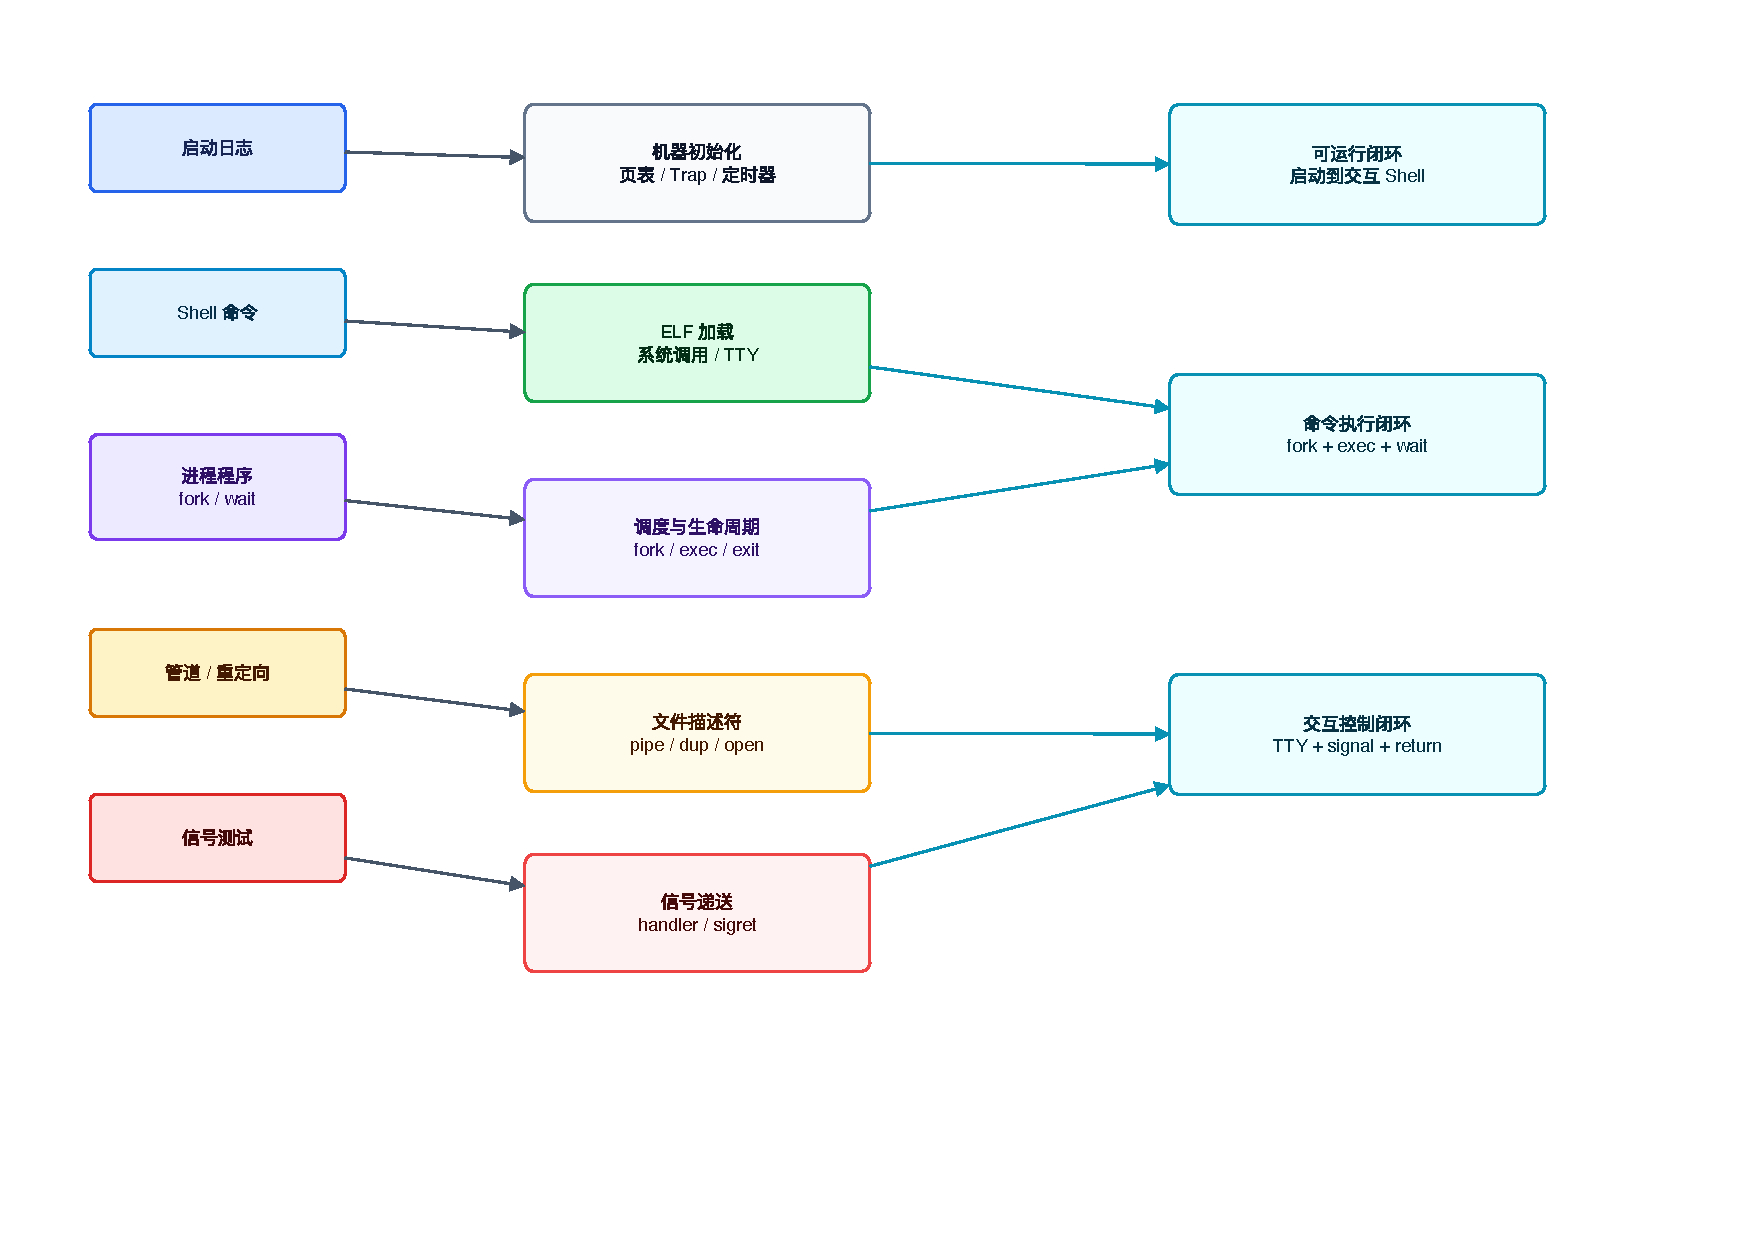
\includegraphics[width=0.95\textwidth]{figures/validation-matrix.pdf}
  \caption{系统功能验证覆盖关系}\label{fig:validation-matrix}
\end{figure}

\figref{fig:validation-matrix} 将测试对象和内核模块对应起来。启动测试覆盖机器初始化、内存管理、Trap 和文件系统挂载；Shell 命令覆盖用户程序加载、系统调用和 TTY；进程类程序覆盖调度与父子进程；管道和重定向覆盖文件描述符与进程协作；信号测试覆盖 TTY、异常和用户态上下文恢复。这些测试尚不能替代完整自动化测试体系，但对于教学操作系统移植而言，可以确认系统已经具备从启动到交互、从命令执行到进程回收的基本运行路径。

\begin{table}[htbp]
  \centering
  \caption{建议补充的运行截图与测试材料}\label{tab:screenshot-placeholders}
  \renewcommand{\arraystretch}{1.25}
  \begin{tabular}{p{0.24\textwidth}p{0.38\textwidth}p{0.26\textwidth}}
    \toprule
    材料 & 建议运行内容 & 论文中对应位置 \\
    \midrule
    启动日志截图 & 执行 \verb|make qemu-riscv64|，截取 OpenSBI 后内核初始化和 Shell 提示符出现的终端输出 & 启动与运行环境验证 \\
    Shell 命令截图 & 在 Shell 中运行 \verb|ls|、\verb|mkdir|、\verb|echo|、\verb|cat|、\verb|rm| 等命令 & 文件接口与用户程序验证 \\
    进程测试截图 & 运行 \verb|fork| 或 \verb|forks|，截取父子进程输出和返回 Shell 的结果 & 进程生命周期验证 \\
    管道与重定向截图 & 运行 \verb|echo hello > a|、\verb|cat a| 或等价管道命令 & 文件描述符和 Shell 解析验证 \\
    信号测试截图 & 运行 \verb|sig|、\verb|newsig| 或在前台程序中输入 Ctrl-C & 信号递送和恢复验证 \\
    \bottomrule
  \end{tabular}
\end{table}

\begin{figure}[htbp]
  \centering
  \fbox{\begin{minipage}[c][0.22\textheight][c]{0.88\textwidth}
    \centering
    此处替换为 QEMU 运行截图：建议包含启动日志、Shell 提示符、常用命令、进程测试和信号测试中的至少两类输出。
  \end{minipage}}
  \caption{QEMU 运行与交互测试截图占位}\label{fig:qemu-screenshot-placeholder}
\end{figure}

\section{结果分析}

从构建结果看，当前系统已经形成面向 RISC-V 的构建链。Rust 内核可以以 \verb|no_std| 方式生成 RISC-V ELF，用户库、Shell 和用户程序可以交叉编译为 ELF64/RISC-V，可执行文件和资源可以写入 Unix V6++ 文件系统镜像，QEMU virt 机器可以通过 OpenSBI 加载内核并挂载 VirtIO 磁盘。上述结果表明，重构工作覆盖了内核语言迁移、用户态程序、镜像制作和仿真运行等工程环节。

功能结果显示，当前系统相较 \verb|main| 分支完成了三类迁移。体系结构由 IA-32/PC 迁移到 RISC-V/QEMU virt，启动、中断、系统调用、页表和设备访问路径均发生变化。内核主体由 C++ 改写为 Rust，进程、文件对象、文本段引用、中断保护等资源的生命周期表达更明确，错误返回也更多通过 \verb|Result| 和枚举呈现。用户态环境保持 Unix V6++ 的 Shell 和常用命令语义，原教学系统的使用方式得以延续。

当前验证仍以手工交互和模块级观察为主，自动化程度有限。文件系统和 Buffer 管理虽然可以支撑基本命令与镜像访问，但其内部一致性、异常恢复和压力场景仍需要更系统的测试；进程退出状态、子进程时间累计等细节仍有简化；部分系统调用保留为空实现或返回 \verb|ENOSYS|。这些限制不影响本文所述的 RISC-V/Rust 移植主线，也说明系统仍处于教学内核的可运行框架阶段，后续需要继续补充自动化测试、压力测试和更完整的 Unix 语义。

\section{结论与展望}

本文围绕 Unix V6++ 教学操作系统面向 RISC-V 平台的移植与 Rust 重构展开研究。在保持 Unix V6++ 原有教学语义和用户态使用方式的基础上，系统将重构前 \verb|main| 分支中面向 IA-32/C++/PC 设备模型的内核，迁移为面向 RISC-V/QEMU virt 平台的 Rust 内核，并完成启动、地址空间、中断异常、系统调用、进程管理、设备适配、Shell 交互和构建验证等工作。

平台迁移完成了 RISC-V 裸机内核的启动流程设计。系统通过 QEMU/OpenSBI 进入位于 \verb|0x80200000| 的内核入口，完成早期栈设置、BSS 清零、串口输出、链接脚本适配和初始化顺序组织；随后基于 Sv39 分页机制建立内核高地址映射、用户地址空间映射和 MMIO 设备映射，并通过 \verb|satp| 与 \verb|sfence.vma| 启用地址空间保护。物理内存管理保留内核页和用户页划分思想，接入 Buddy 分配器、slab 分配器和 Rust 全局分配器，为内核对象、用户进程图像和内核栈分配提供页级资源。

内核事件处理部分基于 RISC-V 特权架构重写了 Trap 框架。系统使用 \verb|stvec| 建立统一入口，通过汇编保存寄存器和关键控制状态，再由 Rust 层根据 \verb|scause| 分发系统调用、时钟中断、外部中断和异常。系统调用接口从原 x86 寄存器约定迁移到 RISC-V \verb|a0| 至 \verb|a7| 的参数传递方式，用户态 C 库通过 \verb|ecall| 进入内核，内核保留 Unix V6++ 的主要系统调用编号和语义。时钟中断、PLIC 外部中断和 UART 输入路径接入后，调度、TTY 和信号处理可以在新平台上配合运行。

进程管理和用户程序支持实现了进程控制块、进程状态机、优先级调度、睡眠唤醒、上下文切换以及 \verb|fork|、\verb|exec|、\verb|exit|、\verb|wait| 等核心进程系统调用。相较 \verb|main| 分支中的固定进程数组、x86 上下文和 PE 用户程序格式，当前系统使用 RISC-V \verb|TrapContext| 与 \verb|TaskContext| 表达用户态返回和内核态切换，使用 ELF64/RISC-V 作为主要用户程序格式，并由 \verb|exec| 完成程序段加载、用户栈构造和 argc/argv 传递。信号机制也迁移到 RISC-V 上下文模型下，可支持终端控制字符、用户发送信号和部分用户态异常到信号的转换。

Rust 重构重新表达了教学内核中的资源管理边界。当前系统仍然保留裸机内核不可避免的底层操作，例如页表项修改、MMIO 访问、用户指针读取和汇编上下文切换；在这些必要的 \verb|unsafe| 边界之外，页资源、内核栈、文本段引用、inode 引用、文件引用和中断开关保护等对象更多通过所有权、生命周期、\verb|Drop| 和 RAII 风格封装表达。原 C++ 版本中不少资源释放依赖调用路径上的显式配对操作，当前 Rust 版本把部分释放责任收束到类型本身，使读者在追踪进程退出、文件关闭和页回收时更容易看到资源由谁持有、何时释放。

当前系统已经具备教学内核所需的基本运行路径，但仍存在一些可以继续完善的问题。测试体系仍以构建检查、启动日志观察和 QEMU 中的交互式功能测试为主，自动化程度有限。后续可以围绕系统调用、进程生命周期、文件描述符、管道、信号和异常处理建立更系统的用户态测试集，并把测试程序纳入镜像生成和 QEMU 自动运行流程，使每次修改都能得到更明确的回归反馈。部分 Unix 语义仍有简化空间，例如若干系统调用尚未完整实现，\verb|wait| 对子进程退出状态和时间统计的处理也较简化，信号机制尚未覆盖更完整的屏蔽、排队和默认动作细节。后续可在不破坏教学内核规模的前提下，逐步补齐这些接口，使用户态程序的行为更加接近 Unix 传统语义。

本文完成了 Unix V6++ 从 IA-32/C++/PC 设备模型到 RISC-V/Rust/QEMU virt 平台的主要迁移与重构工作，保留了原教学系统的 Unix 风格语义和用户态交互方式，并形成了可构建、可运行、可测试的教学操作系统框架。当前系统还未达到通用操作系统的功能完备程度，但已经能够作为理解 RISC-V 操作系统机制、Rust 内核资源管理和 Unix V6++ 教学语义迁移的实践载体。后续工作可以继续推进自动化测试、系统调用完整性、异常场景验证和教学实验化，使该系统更适合长期维护和课程使用。
